%%%%%%%%%%%%%%%%%%%%%%%%%%%%%%%%%%%%%%%%%%%%%%%%%%%%%%%%%%%%%%%
%
% Welcome to writeLaTeX --- just edit your LaTeX on the left,
% and we'll compile it for you on the right. If you give
% someone the link to this page, they can edit at the same
% time. See the help menu above for more info. Enjoy!
%
%%%%%%%%%%%%%%%%%%%%%%%%%%%%%%%%%%%%%%%%%%%%%%%%%%%%%%%%%%%%%%%

% --------------------------------------------------------------
% This is all preamble stuff that you don't have to worry about.
% Head down to where it says "Start here"
% --------------------------------------------------------------
 
\documentclass[12pt]{article}
 
\usepackage[margin=1in]{geometry}
\usepackage{amsmath,amsthm,amssymb}

\usepackage{listings}
\usepackage{xcolor}

\usepackage{tikz}
\usetikzlibrary{shapes,positioning}

\tikzset{ell/.style={circle,draw,minimum height=0.2cm,minimum width=0.2cm,inner sep=0.15cm}}

%New colors defined below
\definecolor{codegreen}{rgb}{0,0.6,0}
\definecolor{codegray}{rgb}{0.5,0.5,0.5}
\definecolor{codepurple}{rgb}{0.58,0,0.82}
\definecolor{backcolour}{rgb}{0.95,0.95,0.92}

%Code listing style named "mystyle"
\lstdefinestyle{mystyle}{
  backgroundcolor=\color{backcolour}, commentstyle=\color{codegreen},
  keywordstyle=\color{magenta},
  numberstyle=\tiny\color{codegray},
  stringstyle=\color{codepurple},
  basicstyle=\ttfamily\footnotesize,
  breakatwhitespace=false,         
  breaklines=true,                 
  captionpos=b,                    
  keepspaces=true,                 
  numbers=left,                    
  numbersep=5pt,                  
  showspaces=false,                
  showstringspaces=false,
  showtabs=false,                  
  tabsize=2
}

%"mystyle" code listing set
\lstset{style=mystyle}

 
\newcommand{\N}{\mathbb{N}}
\newcommand{\Z}{\mathbb{Z}}
 
\newenvironment{theorem}[2][Theorem]{\begin{trivlist}
\item[\hskip \labelsep {\bfseries #1}\hskip \labelsep {\bfseries #2.}]}{\end{trivlist}}
\newenvironment{lemma}[2][Lemma]{\begin{trivlist}
\item[\hskip \labelsep {\bfseries #1}\hskip \labelsep {\bfseries #2.}]}{\end{trivlist}}
\newenvironment{exercise}[2][Exercise]{\begin{trivlist}
\item[\hskip \labelsep {\bfseries #1}\hskip \labelsep {\bfseries #2.}]}{\end{trivlist}}
\newenvironment{problem}[2][Problem]{\begin{trivlist}
\item[\hskip \labelsep {\bfseries #1}\hskip \labelsep {\bfseries #2.}]}{\end{trivlist}}
\newenvironment{question}[2][Question]{\begin{trivlist}
\item[\hskip \labelsep {\bfseries #1}\hskip \labelsep {\bfseries #2.}]}{\end{trivlist}}
\newenvironment{corollary}[2][Corollary]{\begin{trivlist}
\item[\hskip \labelsep {\bfseries #1}\hskip \labelsep {\bfseries #2.}]}{\end{trivlist}}

\newenvironment{solution}{\begin{proof}[Solution]}{\end{proof}}
 
\begin{document}
 
% --------------------------------------------------------------
%                         Start here
% --------------------------------------------------------------
 
\title{Quiz 2}%replace X with the appropriate number
\author{Mengxiang Jiang\\ %replace with your name
CSEN 5336 Analysis of Algorithms} %if necessary, replace with your course title
 
\maketitle
 
\begin{problem}{1} %You can use theorem, exercise, problem, or question here.  Modify x.yz to be whatever number you are proving
    The pattern $P$, alphabet $\Sigma$ and text $T$ is given for a string matching problem. Find the
state transition diagram, state transition table and current state values ($q$) to find
matched pattern in the text and find the valid shifts.\\\\
$P=$ bcbca\\
$\Sigma =$ \{a, b, c, d\}\\
$T=$ bcbcdbcbcbcad\\\\
State transition diagram:\\
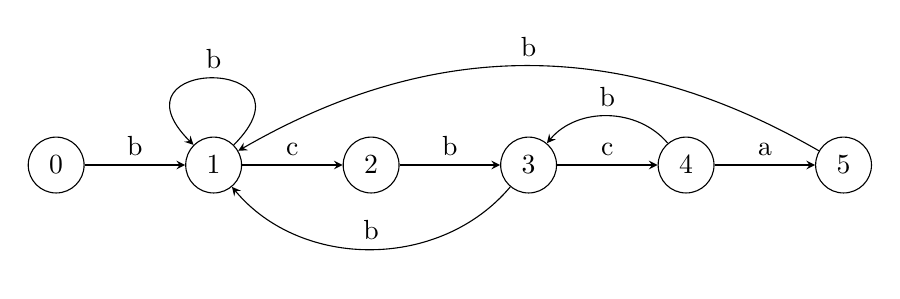
\begin{tikzpicture}[>=stealth]
    \node[ell] (s1) at (0,0) {0};
    \node[ell] (b1) at (2,0) {1};
    \node[ell] (c1) at (4,0) {2};
    \node[ell] (b2) at (6,0) {3};
    \node[ell] (c2) at (8,0) {4};
    \node[ell] (a1) at (10,0) {5};

    \draw [->] (s1) to []node[above]{b} (b1);
    \draw [->] (b1) to []node[above]{c} (c1);
    \draw [->] (b1) to [loop]node[above]{b} (b1);
    \draw [->] (c1) to []node[above]{b} (b2);
    \draw [->] (b2) to []node[above]{c} (c2);
    \draw [->] (b2) to [bend left=50]node[above]{b} (b1);
    \draw [->] (c2) to []node[above]{a} (a1);
    \draw [->] (c2) to [bend right=50]node[above]{b} (b2);
    \draw [->] (a1) to [bend right]node[above]{b} (b1);
\end{tikzpicture}
\\State transition table:\\\\
\begin{tabular}[b]{|c|c|c|c|c|} 
  \hline
  State & a & b & c & d \\
  \hline
  0 & 0 & 1 & 0 & 0\\
  \hline
  1 & 0 & 1 & 2 & 0\\
  \hline
  2 & 0 & 3 & 0 & 0\\
  \hline
  3 & 0 & 1 & 4 & 0\\
  \hline
  4 & 5 & 3 & 0 & 0\\
  \hline
  5 & 0 & 1 & 0 & 0\\
  \hline
\end{tabular}
\\Current state values:\\\\
\begin{tabular}[b]{|c|c|c|c|c|c|c|c|c|c|c|c|c|c|c|} 
  \hline
  i & 0 & 1 & 2 & 3 & 4 & 5 & 6 & 7 & 8 & 9 & 10 & 11 & 12 & 13 \\
  \hline
  T[i] &  & b & c & b & c & d & b & c & b & c & b & c & a & d\\
  \hline
  q & 0 & 1 & 2 & 3 & 4 & 0 & 1 & 2 & 3 & 4 & 3 & 4 & 5 & 0\\
  \hline
\end{tabular}
\\one valid shift at i = 12 $\rightarrow$ shift of i - m = 12 - 5 = 7.
\end{problem}

% --------------------------------------------------------------
%     You don't have to mess with anything below this line.
% --------------------------------------------------------------
 
\end{document}